\section{Plasma}
	\label{sec:plasma}
	This section presents a short overview of basic plasma theory, it can serve as a
	quick reminder if already familiar with the subject, and necessary
	background to understand the numerical simulations in this work.
    % If you, the reader, is already familiar with plasma physics this section could serve as
    % as a quick reminder about important basic plasma theory. Or it could hopefully
    % serve as a too short and shallow introduction, to the uninitatied reader,
    % of the knowledge needed to make sense of the numerical experiments in this
    % thesis.
	For a more thorough introduction the books \textit{\citetitle{fitzpatrick_plasma_2014}}
    \citep{fitzpatrick_plasma_2014}, \textit{\citetitle{goldston_introduction_1995}} \citep{goldston_introduction_1995},
    \textit{\citetitle{pecseli_waves_2012}} \citep{pecseli_waves_2012} or the classic
    \textit{\citetitle{chen_introduction_1984}} \citep{chen_introduction_1984} can be consulted.

	Plasma is the fourth, lesser known, state of matter. It is similar to a gas
	in that the particles are free to move, but it has the key distinction that
	a part of its constituent particles are electrically charged.
	\\[1.0cm]
	\indent \textit{\large"A plasma is a quasineutral gas of charged and neutral particles which exhibits
	collective behaviour."}
	\begin{flushright}
	    \textbf{Francis F. Chen}\\[1.0cm]
	\end{flushright}
	The charge causes the particles to be subject to the Lorentz force, which
	changes the behaviour of the gas. The plasma state is a typical state of matter
	and can be found in;
	sun/stars, northen light, plasma cutters (Welding arcs), argon light tubes, fusion, a lot of various
	industrial techniques, earth athmosphere. (Make this into a paragraph)

	Plasma are fun because of (Intriguing physics, useful for industrial applications,
	solar storms, the ever elusive fusion, space craft, predicting solar storms)

	\begin{figure}
		\begin{center}
			% 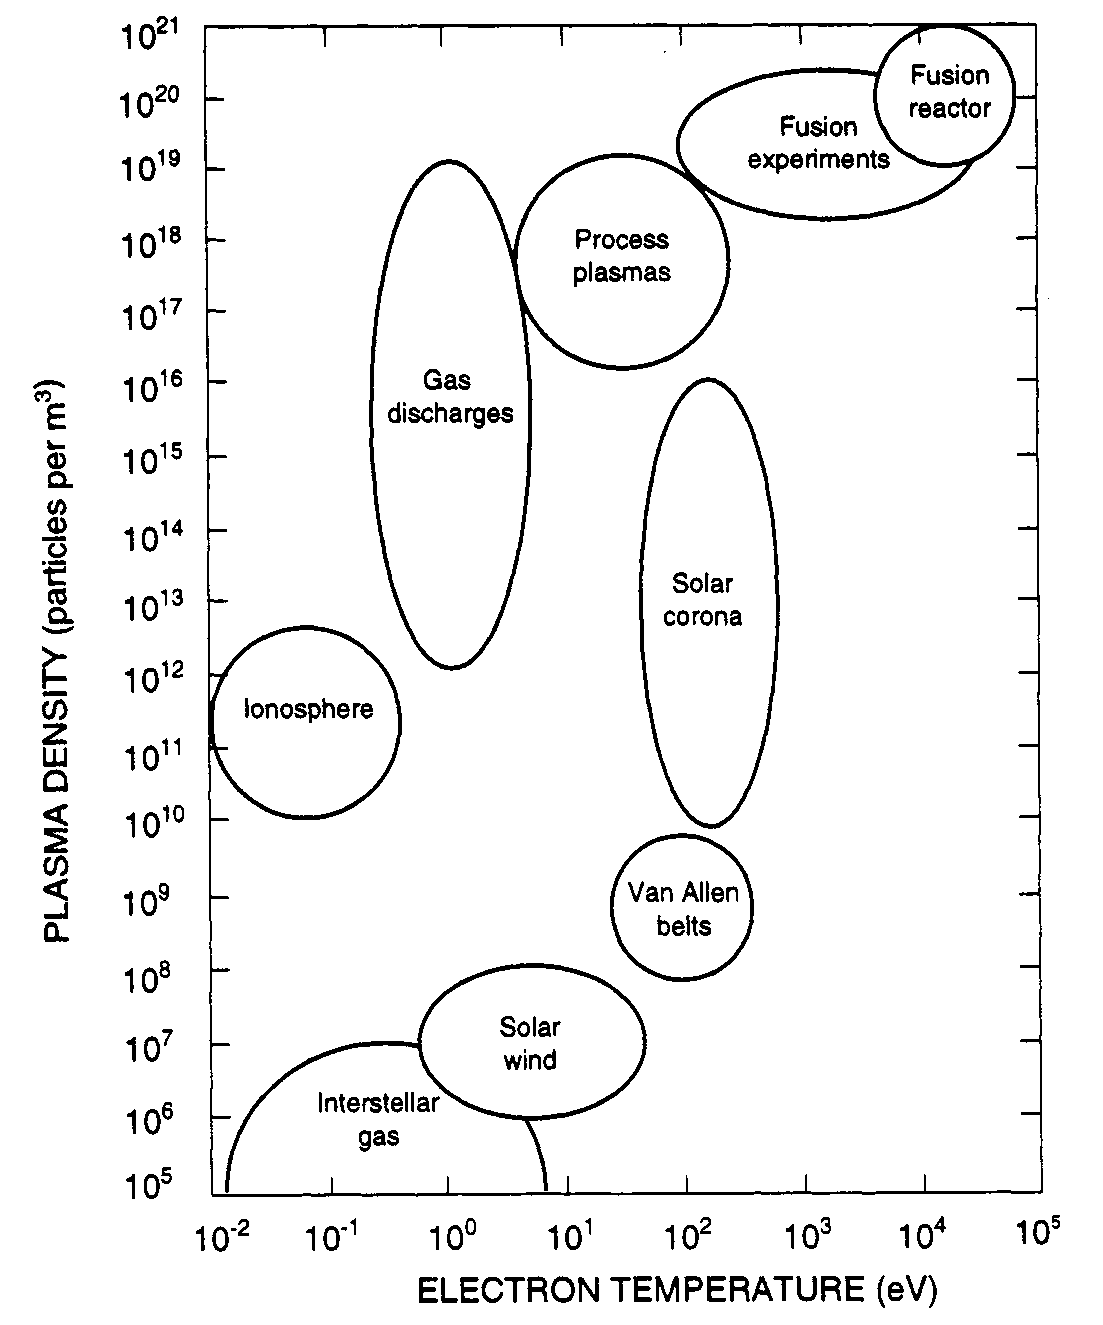
\includegraphics[width = 0.5\textwidth]{figures/theory/plasma_density}
			\missingfigure[figwidth=\textwidth]{Plasma Regimes}
		\end{center}
		\caption{Plasmas occurs both in the hot and dense condiotions in necessary for fusion, as
		well as in the cold and sparse interstellar environment. [NOTE MAKE BETTER FIGURE]
		}
	\end{figure}



    \subsection{Plasma Parameters}
		\label{sec:parameters}
		\subsubsection{Temperature}
		A modern view of temperature comes from kinetic theory developed by
		Maxwell and Boltzmann \citep{swendsen_statistical_2006}. We will not go through it
		here but a treatment is available in \citet{goldston_introduction_1995}.
		Temperature is then related to the average kinetic energy of a particle.
		For an ideal monoatomic gas the kinetic energy is then

		\begin{equation}
			\bar{E}_k = \frac{1}{2} m v_{th}^2 = \frac{3}{2} kT \label{eq:temperature}
		\end{equation}

		Here we have introduced \(v_{th} \equiv  \sqrt{kT/m}\) as the thermal velocity, i.e.
		the average velocity of a particle. It should be mentioned that the fraction in
		front of the temperature is dependent on the degrees of freedom of the particle.
		A monoatomic particle can only move in three directions, but a diatomic particle
		can also vibrate and spin. (Correct?)

		In high energy plasma physics it is also costumary to drop the Boltzmann factor, \(k\),
		in \cref{eq:temperature}, and express temperature directly in electronvolt, \(eV\).
		Electronvolt is defined as the energy it takes to move an elementary charge through
		a potential difference of \(1\) \si{\volt}, and corresponds to approximately
		\(11600 \si{\kelvin}\). For the space and atmospheric plasmas, we are mostly
		dealing with here, the temperatures are generally low, so we will use the Kelvin scale
		for temperature.

		If the particles in a plasma collide often compared to the characteristic timescales
		of energy and particle changes, the particle velocity distribution can be approximated
		by a Maxwellian distribution. It is only then that the concept of
		temperature is valid \citep{goldston_introduction_1995}.

		\subsubsection{Electron Plasma Frequency}
		A rather important frequency in plasma physics is the electron plasma frequency,

		\begin{equation}
			\omega_{pe} \equiv \sqrt{\frac{ne^2}{\epsilon_0 m_e}}
		\end{equation}

		This frequency, \(\omega_{pe}\), is dependent on the number density, \(n\),
		the fundamental charge, \(e\), the vacuum permittivity, \(\epsilon_0\), and
		the electron mass, \(m_e\).
		It can be thought of as a typical electrostatic oscillatory frequency.
		Consider an electrically neutral 1D slab, which is then disturbed, from its
		neutrality, by an infinitesimal charge density on one side.

		\begin{equation}
			\sigma = en\delta x
		\end{equation}

		It will have an equal and opposite charge density on the other side. The slab
		will then have an electric field due to the charge density, caused by Gauss' Law.

		\begin{equation}
			\pdv{E_x}{x} = -\frac{\sigma}{\epsilon_0} \qquad\rightarrow\qquad
			E_x = \frac{-en\delta x}{\epsilon_0}
		\end{equation}

		Inserting this field as the only force in Newtons law for a single particle yields

		\begin{equation}
			m\pdv{\delta x}{t} = eE_x = -m\omega_{pe}^2\delta x
		\end{equation}

		The particle will then oscillate around its equilibrium position with
		the electron plasma frequency. The same phenomen often happens in plasma as
		it tries to go back to its equilibrium and is called plasma oscillations,
		or Langmuir oscillations, see \cref{sec:langmuir} for a treatment of plasma oscillations.

		An otherwise useful timescale is the reciprocal of the plasma frequency,
		the plasma period

		\begin{equation}
			\tau_p \equiv 2\pi/\omega_{pe}
		\end{equation}

		Some researchers prefer to define the \(\tau_p\), without the \(2\pi\) prefactor,
		as that makes some concepts neater.

		\subsubsection{Debye Shielding}
		Debye shielding length is the distance at which the electric influence
		from a particle is shielded out by the surrounding plasma.
		Consider a charged particle immersed in a plasma bath. The plasma is in
		a thermodynamical equilibrium, i.e. there is no significant temperature
		gradients. We artificially place a positively charged ion into the plasma.
		This ion will then attract electrons and repel positive ions. There will be a tendency
		for there to be more negativily charged particles, and less positive, near the
		ion, which in effect will work as an electric shield around the ion. The
		distance away from a particle where its field, is typically mostly cancelled
		out is called the Debye Shielding Length, \(\lambda_D\).

		\begin{equation}
			\lambda_D \equiv \sqrt{\frac{\epsilon_0 kT_e}{n_e e^2}}
		\end{equation}

		The above definition is often used, \citep{pecseli_waves_2012},
		neglecting the ion influence since they often have a much lower temperature.
		The shielding length is dependent on the ratio between temperature, \(T_e\),
		and electron density, \(n_e\).
		In cases where we also need to account for ions, a more complete definition can be used

		\begin{equation}
			\lambda_D \equiv \sqrt{\frac{\epsilon_0 k T_e}{n_e e^2(1+Z \frac{T_e}{T_i})}}
		\end{equation}

		Due to the earlier argument, and the statistical approach used when deriving it \citep{goldston_introduction_1995},
		there must be a significant amount particles close to the ion to shield it out.

		It should be noted that the shielding length is related \citep{fitzpatrick_plasma_2014} to the
		the plasma period and the thermal velocity through

		\begin{equation}
			\lambda_D \propto \tau_p v_{th}
		\end{equation}


		\subsubsection{Quasineutrality}
		The assumption of quasi-neutrality is a common approximation in plasma
		physics. By quasi-neutrality we assume that the electron
		density is equal to the ion density, \(n_e \approx n_i\). This is often called the
		\textit{"plasma approximation"} \citep{chen_introduction_1984}.
		This approximation is usually valid on length scales much larger than the shielding
		length. If we had a case where a large volume of plasma lost a significant
		amount of charge, a large electric field would accompany the density imbalance.
		This electric field would quickly correct the imbalance, and quasineutrality
		would be regained.

		\subsubsection{Plasma Classification}
        For a plasma description to be useful the system we consider must have
        a typical length scale, \(L\), and time scale, \(\tau\), larger than the Debye length and plasma
        period respectively.

        \[\frac{\lambda_D}{L} \ll 1  \qquad{} \qquad \frac{\tau_p}{\tau} \ll 1 \]


















%Stay here fucker
